%************************************************
\chapter{All Things Classical}\label{chap:compilers}
%************************************************

In this chapter we will give a very brief overview of the components of classical computers that will be helpful to further discussions of quantum circuit compilation.
A key component to quantum circuit compilation is the word ``compilation'' whose origins (in computing) date to the early 1950's when electronic digital computers were in their early stages.
Understanding the historical development of compilation and its techniques will provide ideas and tools necessary to solve the new task of quantum circuit compilation.

This chapter is meant to provide the reader with the basics of some computing terminology and ideas.
It is by no means a complete introduction to compilers, nor computer architecture.

\section{What can a computer do?}

If you're reading this, I'm sure you can imagine something your computer is capable of.
Maybe reading this document online, sending messages/email, browsing the internet, writing documents, etc.
These are very high level operations our computer can perform, but under the hood much more primitive operations are taking place.
It is these primitive operations that we wish to understand, and will have many similarities with modern-day quantum hardware.

A simplified model of computer architecture, known as the von Neumann Architecture (\cref{fig:comparch}) shows what we now call a \ac{CPU} which is the workhorse of the computer.\footnote{At least in this \emph{very simplified} model.}

\begin{figure}[h]
    \centering
    \includestandalone[width=0.8\textwidth]{tikz/arch}
    \caption{von Neumann Architecture scheme}\label{fig:comparch}
\end{figure}

Since the \ac{CPU} is the computational component of the computer, what can \emph{it} do?
Modern \acp{CPU} are built on the \ac{ISA} which means that the \ac{CPU} has a finite set of operations or instructions that it can perform.
Every operation the computer can perform must be built up from these primitive instructions.
Some examples of what these primitive operations might be are:
\begin{itemize}
    \item put a value into memory;
    \item add two values in memory together and store the result in a new location;
    \item perform the bitwise negation on a value;
    \item compute the square root of a value.
\end{itemize}
One can then use these primitives to build up complex functionality that eventually implement the capabilities we know and love (and hate) computers for.
By choosing an \ac{ISA}, a \emph{complexity class} is created of all the problems that can be solved using a polynomial number of instructions.\footnote{Polynomial refers to the function which takes the \emph{size} of the problem input, and returns the number of steps (or time) required to solve the problem.}
In practice most \acp{ISA} implement the same complexity class which we denote by P and refers to decision problems solvable by a deterministic Turing machine in a polynomial amount of time. % TODO complexity
There are many \acp{ISA} one can come up with that spawn different complexity classes, of which the ones we expect some familiarity with are P and NP on the classical side, and BQP on the quantum side.
For more details on complexity classes consult~\cite{complexity} and~\cite[Chapter 3]{nielsenchuang}.

The \ac{ISA} architecture style has seen major success, but it suffers from the drawback of requiring the programmer to work at the very low level of machine instructions.
To work at a higher level of abstraction, and hence to have a higher-level of productivity, computer scientists and programmers created new languages which were easier to read, write, and reason about.
This necessitated new languages to be ``translated'' into the instruction set after the code was written.
The software responsible for translating these higher level ideas into a machines instruction set are known as \textbf{compilers}.

\section{Compilers}

While compilers have their origins in the aforementioned translation of higher-level code into lower-level code, they have grown considerably to perform many more tasks.
Before we dive into all of the capabilities of modern compilers, let's take a step back and recall what the word compile means.

Merriam-Webster~\cite{compiledef} defines the word \emph{compile} to mean
\begin{quote}
    to compose out of materials from other documents.
\end{quote}
In the context of programming language compilers,  ``other documents'' might mean the code itself, as well as configuration files and environment variables.
With these materials the lower level machine code is then composed.
This definition is reflected in~\citetitle{dragonbook}\footnote{Colloquially known as ``The Dragon Book'' because of the cover, and likely the most famous book on (classical) compilers. This is also where the logo of the LLVM project originates from which we will discuss in~\cref{sec:llvm}.}\graffito{
    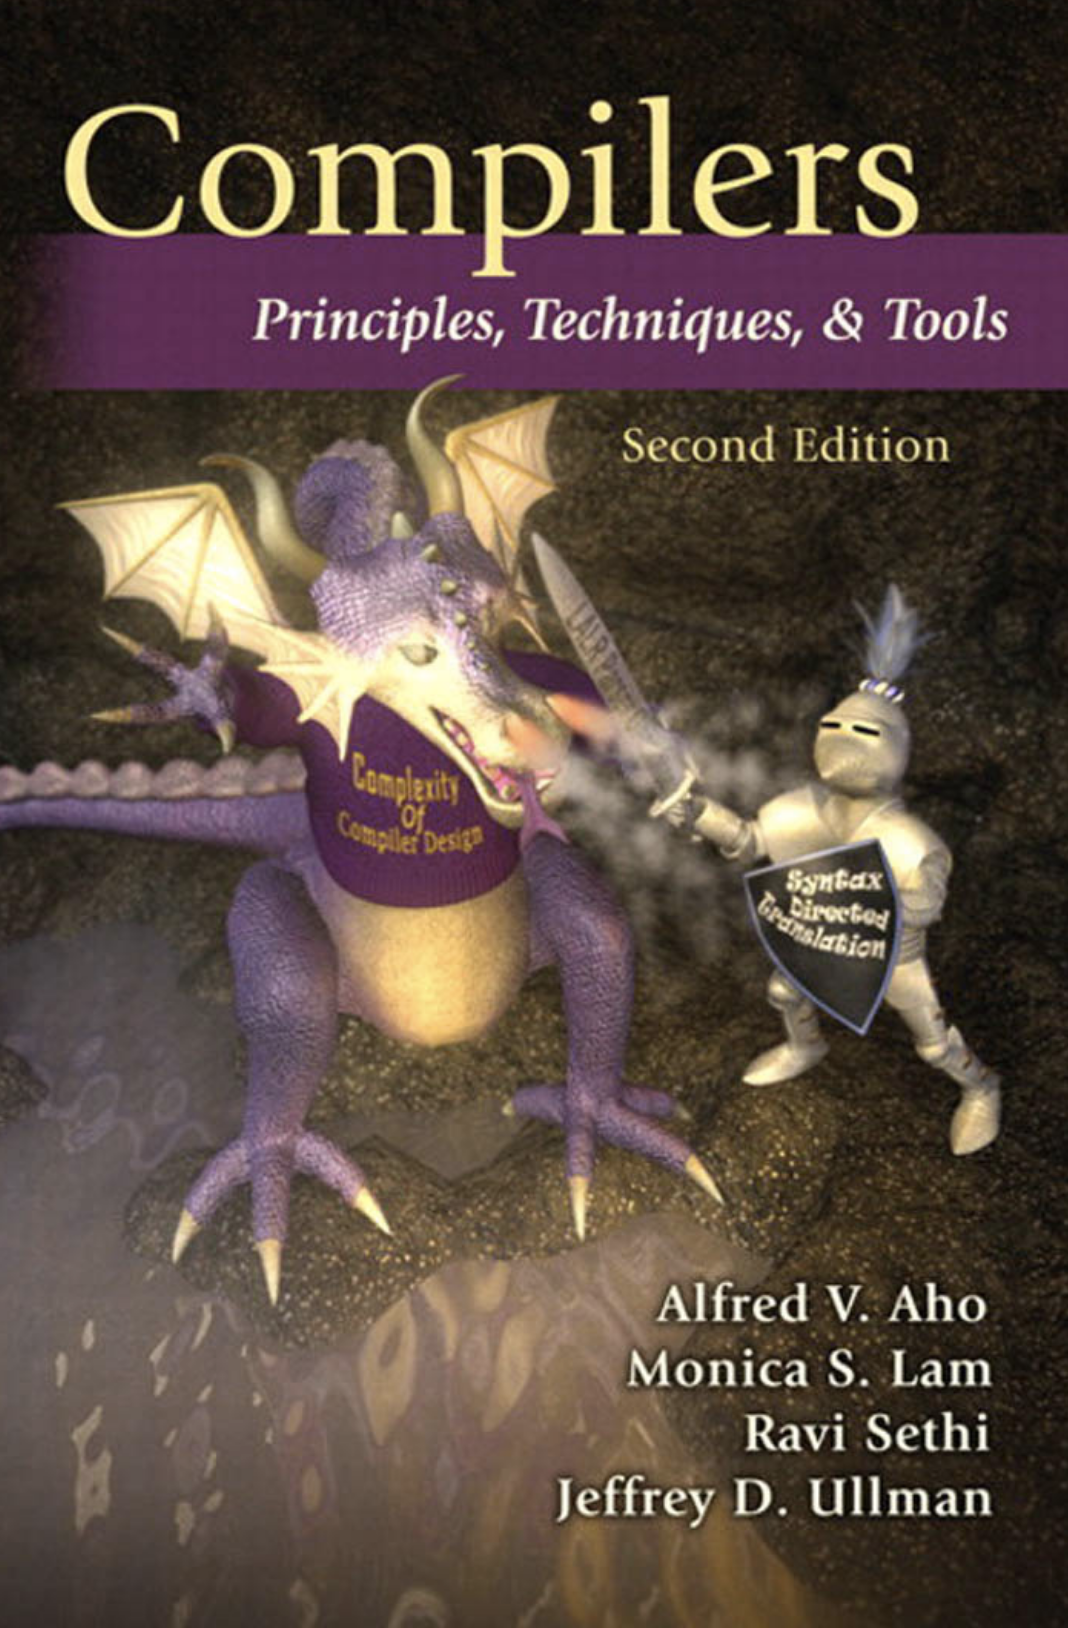
\includegraphics[width=\marginparwidth]{img/dragonbook.png}
    \emph{The Dragon Book}
    
\includegraphics[width=\marginparwidth]{img/llvmlogo.png}
    \emph{LLVM Logo}
}~\cite{dragonbook} where the authors introduce compilers through the process of transforming software.
\begin{quotation}
    [B]efore a program can be run, it first must be translated into a form in which it can be executed by a computer.

    The software systems that do this translation are called \emph{compilers}.
\end{quotation}
Hence we can view compilers as a function taking software written at one level of abstraction and bringing it down to a lower level that a computer's \ac{CPU} can understand.
\begin{figure}[ht]
    \centering
    \includestandalone[width=0.8\textwidth]{tikz/compiler}
    \caption{Action of Compiler}\label{fig:compiler}
\end{figure}

The term compiler was first used in the context computers by Grace Hopper in the early 1950's while working on a system that could translate symbolic mathematics into a machine language.
Initially Hopper's new idea was met with resistance as it was thought to be unrealistic.
\begin{quotation}
    I had a running compiler, and nobody would touch it because, they carefully told me, computers could only do arithmetic; they could not do programs.
    It was a selling job to get people to try it.
    I think with any new idea, because people are allergic to change, you have to get out and sell the idea.
    \attrib{Grace Hopper~\cite{hopperquote}}
\end{quotation}
In the end she succeeded in selling the idea and compilers have become a ubiquitous piece of modern computing infrastructure.
While Hopper's compiler focused solely on code translation, a modern compiler might perform all of line reconstruction, preprocessing, lexical analysis, syntax analysis, semantic analysis, conversion to an \ac{IR}, optimization (and there are many different types!), and finally code generation.
Thankfully we will not need to understand \emph{all} of these parts in full, but rather will focus on \aclp{IR}, optimizations, and code generation.

\subsection{Compilation Phases}\label{sec:comp-phases}

As alluded to in the previous section, a compiler has many different responsibilities.
Each responsibility is broken into a separate component so that it can be understood on its own.
A schematic for this can be seen in~\cref{fig:compilerphases} for the main steps that we will be concerned with in this document.
\begin{wrapfigure}[24]{i}{0.25\textwidth}% TODO tweak lineheight
    \centering
    \includestandalone[width=0.23\textwidth]{tikz/phases}
    \caption{Compiler Phases}\label{fig:compilerphases} % TODO can we fix this caption?
\end{wrapfigure}

\paragraph{Syntax Analyzer}
This phase is for ensuring the code is syntactically well formed (that is, that it abides by the specification of the language).
If one is writing code in a binary alphabet with characters \texttt{0} and \texttt{1}, then the ``program'' \texttt{00011} is syntactically valid, while \texttt{1102} is not because a \texttt{2} appears in the code.
Many compilers transform the code into a syntax tree to complete the verification.

\paragraph{Semantic Analyzer}
Now that the code is syntactically valid, we can ensure it has meaning.
This phase usually consists of type checking and scope validation (ensuring the code does not access variables outside of scope).
In many compiled languages the operation \texttt{'hello' * 5} would pass syntax analysis, but fail semantic analysis because a string multiplied by an integer is not a valid operation.\footnote{It is completely valid in other languages like Python, but Python is not a compiled language.}

\paragraph{Intermediate Code Generator}
The code is now ensured to be well formed and can begin preparation to execute on hardware.
Passing directly to the code generator is possible from here, but the end product will be slower as no optimizations will take place.
Instead, the existing code (or sometimes using the syntax tree created in the previous steps) will be transformed into an \acf{IR}.
This is a mid-level representation of the code in that it is typically thought of as somewhere between the high level of abstraction of the programming language, and the low level instruction set.

This is best seen with a simple example.
Suppose we have the following snippet to calculate the final location of a moving object after 5 seconds.
\begin{lstlisting}
    x_final = x_initial + velocity * 5
\end{lstlisting}
Upon transforming this code to an \ac{IR}, it takes on a more basic form.
\begin{lstlisting}
    t1 = inttofloat(5)
    t2 = velocity * t1
    t3 = x_initial + t2
    x_final = t3
\end{lstlisting}
The power here comes from the fact that the \acf{IR} can be language agnostic, and hence many languages can compile into the same \ac{IR}.
This design allows for the use of an optimizer for many languages.

\paragraph{Code Optimizer}
Once the code is in the \ac{IR}, the optimizer will attempt to ``improve'' it using many different methods.
Improve can mean many different things, but usually refers to runtime and memory use.
Optimizations that occur during this step are constant propagation, dead code elimination, removing unnecessary code from loops, and loop unrolling.
Optimizing the above example our code is still ``bulkier'' than originally written, but compressed in comparison to the original \ac{IR}-form.
\begin{lstlisting}
    t1 = velocity * 5.0
    x_final = x_initial + t1
\end{lstlisting}
Here we have skipped the call to \texttt{inttofloat} and instead immediately converted the integer \texttt{5} to the float \texttt{5.0}.
We have also combined two of the steps to reduce the number of temporary variables we have to create and store in memory.
As you can see the task of the optimizer is not only to try and speed up the code, but reduce its memory usage as well.
Some of the other problems the code optimizer must tackle are instruction selection, register allocation, and instruction scheduling all of which have analogs we will see in~\cref{chap:circuit-compilers}.

\paragraph{Code Generator}
Finally we have an optimized \ac{IR} and we can generate code for hardware.
This requires us to know which hardware it is we'd like to run our code on as each chip might have a different \ac{ISA}.
This is a very difficult step as many of the sub-problems that are required to be solved are themselves NP-complete such as register allocation~\cite{register-allocation-NP}. % TODO complexity
Further, generating mathematically optimal machine code has also been shown to be undecidable~\cite{dragonbook}!
Hence this step uses effective heuristics to solve the problem at hand in tractable amounts of time.
Typically this step is broken down into first optimizing the \ac{IR} for the hardware that has been chosen, followed by the actual code generation.
If this occurs the optimizer is typically referred to as a hardware-independent optimizer, and a later stage of optimizations is performed in a hardware-dependent optimizer.
We will see later that the distinct phases of optimization are of crucial importance when compiling quantum circuits.

Again following the above code example, upon code generation we may end with the following generic hardware instruction code.

\begin{minipage}{0.5\textwidth}
    \begin{lstlisting}
    LDF R2, velocity
    MULF R2, R2, #5.0
    LDF R1, x_initial
    ADDF R1, R1, R2
    STF x_final, R1
\end{lstlisting}
\end{minipage}
\begin{minipage}{0.5\textwidth}
    \centering
    \begin{tabular}{cc}
        Function      & Meaning         \\ \toprule
        \texttt{LDF}  & Load float      \\
        \texttt{MULF} & Multiply floats \\
        \texttt{ADDF} & Add floats      \\
        \texttt{STF}  & Store float
    \end{tabular}
    \captionof{table}{Machine Code}\label{fig:machcode}
\end{minipage}
Here anything beginning with \texttt{R} is a register.

The phases described here are often grouped into three larger categories.
The syntax and semantic analysis, as well as the generation of an \ac{IR} fall under the umbrella of ``front end'', the optimizer is the optimizer, and everything else that follows is the ``back end''.
The implications of this design is that an optimizer and backend can be paired with many different front ends as long as the front end can generate the optimizer's preferred \ac{IR} flavor.
\begin{figure}[ht]
    \centering
    \includestandalone[width=0.75\textwidth]{tikz/frontback}
    \caption{Compiler with many front and back ends}\label{fig:compends}
\end{figure}

\subsection{Optimizations}

Before moving on to some examples of compilers, its important to understand the separation of concerns in the two types of optimizations we've seen.
The main optimizer we see in~\cref{fig:compilerphases} as ``Code optimizer'' and again the ``Optimizer'' in~\cref{fig:compends} are typically where the majority of optimizations take place in classical compilers and are performed on an \ac{IR}.
One interesting class of examples are peephole optimizations~\cite{classical-peephole}.
These are optimizations that take advantage of small patterns found in code that can be simplified in some way.
Some examples are seen in~\cref{tab:peephole}.
\begin{table}[ht]
    \centering
    \begin{tabular}{p{.5\textwidth}l}
        Instruction                                                      & Optimized Instruction \\ \toprule
        Read value into a register, then immediately store it in memory. & Do nothing            \\
        $a \cdot x + b \cdot x$                                          & $(a + b) \cdot x$     \\
        $x - x$                                                          & $0$                   \\
        $(A^\intercal B^\intercal)^\intercal$                            & $BA$
    \end{tabular}
    \caption{Peephole Optimizations}\label{tab:peephole}
\end{table}
Other examples include dead code elimination, common subexpression elimination, and inlining.
The optimizations done here---usually to the ends of faster runtime and smaller memory use---are performed in the hopes that once the code is compiled into machine code it \emph{will} run faster.
The intuitive optimizations often remove duplication, but many other optimizations that are not so clear take advantage of the commonalities among \ac{CPU} design to produce code that will run faster on any \ac{CPU}.

With an optimized \ac{IR}, and a chosen backend, or hardware, the code can be modified to suit the instruction set, as well as other restrictions the hardware may place on computation.
For example, most \acp{CPU} have a small number of registers, and hence must use them wisely throughout the computation so as to use \emph{all} of them where possible, but not slow down computation by waiting for a register to be available.
Another example is instruction scheduling, where the compiler must figure out an optimal ordering to the computation, again to maximize the \acp{CPU} compute power while not causing bottlenecks.
There are many other examples of hardware-dependent optimizations, but as you might imagine, many require an intimate knowledge of the hardware's particular design.
All this transformation occurs while maintaining the same semantic meaning of the original program.

In summary the first hardware-independent optimization should be thought of as optimizing the implementation theoretically, and the hardware-dependent optimization as ensuring the optimized algorithm runs as fast as possible in its final implementation.
Many more examples of optimizations (both hardware-independent and hardware-dependent) can be found in~\cite[Chapter~8]{compiler-optimizations}.

\subsection{Examples}\label{sec:compiler-examples}

We've now seen what a compiler is and what we typically use it for.
A few examples are in order to help understand how compilers work in the real world, and just how varied they can be.

\begin{description}
    \item[clang:] Short for C Language, this is a compiler frontend for the C/\CPP{} languages. It takes in C/\CPP{} code and produces an LLVM \ac{IR} which we will learn about in~\cref{sec:llvm}. It then lets LLVM handle the rest of the compilation processing.
    \item[Latex:] While perhaps not very obvious, \LaTeX{} is indeed a compiler as it takes high level formatting code, and produces a lower level representation of what the user wants to typeset. Usually that comes in the form of postscript which is another programming language that is read by printers (hardware) to produce the requested document. Postscript can also be read by PDF readers and browsers which then display content as the author desired (maybe).
    \item[TensorFlow:] TensorFlow is a library for machine learning that has drawn on the design principles of compilers in attempts to speed up and ensure the accuracy of models. Indeed it has a frontend where the user builds their model and compiles it into an \ac{IR} known as HLO \ac{IR} or High Level Operations. Typical optimizations then occur and again using the LLVM compiler infrastructure this code can be brought to many backends such as the browser, mobile, and specialized compute infrastructure (such as Google's \ac{TPU}). This is all before we talk about TensorFlow Quantum which allows for hybrid quantum-classical machine learning models~\cite{tensoflowquantum}.
\end{description}

\section{LLVM}\label{sec:llvm}

The LLVM\footnote{The project, while originally an acronym for Low Level Virtual Machine now goes solely by LLVM. The original name reflects the fact that the compiler targets low level \ac{IR} code that runs on some theoretical (hence the term virtual) machine. Since the inception virtual machines have come to mean something different, hence the abandonment of the acronym.} project~\cite{llvm} is one of the largest open source compiler projects in existence and much of the compiler architecture we've discussed here come from its design.
The founder of the project Chris Lattner has characterized compilers succinctly in~\cite{lattnerquote} as
\begin{quote}
    the art of allowing humans to think at a level of abstraction that they want to think about.
\end{quote}

As an interesting historical note, once the \ac{ISA} scheme had become commonplace, chip designers began to implement more and more complex instructions on \acp{CPU} so that machine code became higher level.
At the same time, compilers became more popular, especially as their optimizations became more robust, and useful.
This led to a distinction between chip architectures known as \ac{CISC} and \ac{RISC}.
At the time of writing, \ac{CISC} processors are dominant in desktop computers, while \ac{RISC} processors emphasize efficiency and can be found in phones and many other portable computing hardware.
Some examples include Intel's x86 and x64 chips which are built in the \ac{CISC} style, while ARM is major designer of \ac{RISC} chips (including the most recent Apple Bionic A15 chip). % TODO add note about RISC V?
Today \acp{RISC} are sometimes referred to using the backronym ``Relegate Interesting Stuff to the Compiler''.

With the growth of LLVM, developers have pushed the compiler to extend its use to ``heterogeneous hardware''~\cite{mlir}, which already includes new types of computing hardware like \acp{TPU} and could in the future encompass a \ac{QPU}.
This is exciting not only because classical computer designers are beginning to consider quantum technologies as coprocessors, but because the monumental classical computing infrastructure can then be leveraged to aid in the solutions to quantum problems.
With the futurism, hype, and unknowns surrounding quantum technologies, it often seems that fundamentally new and ingenious ideas are needed to forward the field.
Projects such as the above show there are serious possibilities of recycling, or at the very least, learning from what has come before us.
